\documentclass[main]{subfiles} 


\graphicspath{{img/}}


\begin{document}

\section{Implementation}
The whole project can be found in a repository on GitHub.
There the README will provide the necessary information regarding the implementation of the
scraper as well as how to use the interface.
All the files were written and run in python version $3.9.12$.
Below a list of all the packages plus their respective versions that were used can be found.

\begin{itemize}
    \item \pkg[Scrapy] -  version $2.6.1$
    \item \pkg[Selenium] - version $4.1.5$
    \item \pkg[Webdriver\_manager] - version $3.5.4$
    \item \pkg[Numpy] -  version $1.22.3$
    \item \pkg[Pandas]  - version $1.4.2$
    \item \pkg[Time]
    \item \pkg[Datetime]
    \item \pkg[Openpyxl] - version $3.0.9$
    \item \pkg[Tk (tkinter)] - version $0.1.0$
    \item \pkg[Pillow] - version $9.1.1$
\end{itemize}



\subsection{Structure of the project}
For reference we display the structure of the project below.
Files and directories that do not affect the project directly (such as \pkg[.tex] files)
were not included in the tree.
All of the files in the \pkg[Comparis\_Webscraper] directores except for the ones within the \pkg[spiders]
were set up by \pkg[Scrapy] by default when creating the \pkg[spider].

{ \footnotesize
\begin{forest}
  for tree={
    font=\ttfamily,
    grow'=0,
    child anchor=west,
    parent anchor=south,
    anchor=west,
    calign=first,
    edge path={
      \noexpand\path [draw, \forestoption{edge}]
      (!u.south west) +(7.5pt,0) |- node[fill,inner sep=1.25pt] {} (.child anchor)\forestoption{edge label};
    },
    before typesetting nodes={
      if n=1
        {insert before={[,phantom]}}
        {}
    },
    fit=band,
    before computing xy={l=15pt},
  }
[/.
    [Comparis\_Webscraper
        [Comparis\_Webscraper
            [spiders
                [comparis\_scraper.py]
                [property\_code\_scraper.py]
            ]
            [items.py]
            [middlewares.py]
            [pipelines.py]
            [settings.py]
        ]
        [scrapy.cfg]
    ]
    [data
        [database.xlsx]
        [property\_codes.csv]
        [property\_details.csv]
    ]
    [\textcolor{blue}{\textit{...Continued on next page}}
    ]
]
\end{forest}
}

{ \footnotesize
\begin{forest}
  for tree={
    font=\ttfamily,
    grow'=0,
    child anchor=west,
    parent anchor=south,
    anchor=west,
    calign=first,
    edge path={
      \noexpand\path [draw, \forestoption{edge}]
      (!u.south west) +(7.5pt,0) |- node[fill,inner sep=1.25pt] {} (.child anchor)\forestoption{edge label};
    },
    before typesetting nodes={
      if n=1
        {insert before={[,phantom]}}
        {}
    },
    fit=band,
    before computing xy={l=15pt},
  }
[/.
    [\textcolor{blue}{\textit{...Continued from previous page}}]
    [GUI
        [gui\_data
            [data.xlsx]
            [MeanPriceRooms.xlsx]
            [MeanPriceZip.xlsx]
        ]
        [cleaning\_database.py]
        [graphs\_GUI.py]
        [main.py]
    ]
    [Heatmap
        [PLZO\_SHP\_LV95]
        [MAP1.py]
        [data.xlsx]
    ]
    [README.md]
    [Makefile]
    [.gitignore]
    [.git]
]
\end{forest}
}

\subsection{Implementation of the Web Scraper}
\label{implementationscraper}
As mentioned previously, the web scraping was done by utilizing two different tools, \pkg[Scrapy] and \pkg[Selenium].
When programming the \pkg[spider], the main challenge was to implement the vision of what it should do. 
When called, the \pkg[spider] should be able to do the following:
\begin{enumerate}
    \item Activate the browser via \hspace*{-6pt} \pkg[Selenium]
    \item Access a list of predefined \acsp*{url}
    \item Loop through every \acs*{url} and activate the \jss
    \item Download $22$ datapoints from several locations on the website
    \begin{itemize}
        \item If not available, no value was returned
    \end{itemize}
    \item Process the data via the input processor of the \hspace*{-6pt}\pkg[ItemLoader]
    \item Store data in the \hspace*{-6pt} \pkg[ItemLoader] until the loop has finished
    \item Output (yield) the data from the \hspace*{-5pt} \pkg[ItemLoader] into the "data" directory as \hspace*{-5pt}
    \pkg[.csv] file with the download date in the name
\end{enumerate}

Before explaining how the main spider \pkg[(property\_scraper)] was built,
we provide a brief explanation of how the \acs*{url} of every single property 
was obtained without getting \acs*{ip}-blocked.

\vspace*{5pt}
\subsubsection{Obtaining the List of \acsp*{url}}
\label{scrape1}
Web scraping turned out to be a mix of close investigation of \acs*{html} source codes, 
creative problem solving and a lot of trial and error. 
Obtaining all the property \acsp*{url} was a clear example of this.

Although on a smaller scale, 
it also required a combination of \pkg[Scrapy] and \pkg[Selenium] in order to trigger the JavaScripts.

When a user runs a search on Comparis (e.g. for a house for purchase in a specific location), 
the website will filter through \textbf{all} the listings and return the corresponding properties.
If the user triggers the \js by scrolling, Comparis will load a \acs*{json} 
containing the unique ID's of \textbf{all} search results at the bottom of their \acs*{html}.
This can be seen when right clicking on the page and selecting "Inspect" and entering \pkg[\_\_NEXT\_DATA\_\_] 
in the search field.

\begin{figure}[htbp]
    \centerline{
        
\includegraphics[width = 60mm]{prog_3.png}}
    \caption{Inspect Elements on Browser}
    \label{fig:inspectelement}
\end{figure}

From there on, \pkg[Selenium] will pass the "current state" (i.e. state of \acs*{html} after \js manipulation)
to the spider for the analysis.
The spider then yields the ID's and creates \acsp*{url} by adding them to the end of the \textbf{path component} 
(figure \ref{fig:htmlstructure}) of the \acs*{url}  using an f-string.
This is how Comparis refers to their detail pages.
The data is subsequently saved as \pkg[.csv] to the "data" folder under the name \pkg[property\_codes\_YYYYMMDD.csv].
Adding the current date to the name is necessary with regards to the possibility 
of creating a database that scrapes the web regularly for available real estate.

\begin{figure}[htbp]
    \centerline{
        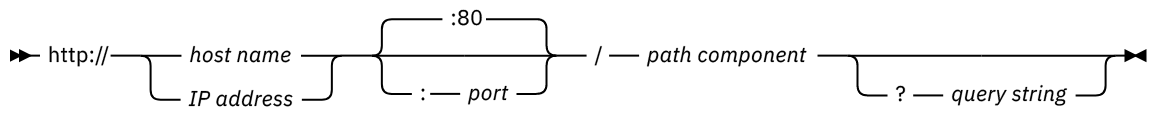
\includegraphics[width = 80mm]{prog_4.png}}
    \caption{Structure of a \acs*{url} \cite{IBMDocumentation2021}}
    \label{fig:htmlstructure}
\end{figure}

\vspace*{5pt}
\subsubsection{Creating the "property-scraper" Spider}
Whilst the idea of combining two different web scraping services into one project came up early on,
a first instance of a working example was presented in an article on towardsdatascience.com\cite{reusovaWebScrapingLess2019}.
However, the given example had to be heavily adapted, especially since in our project, 
using the \pkg[ItemLoader] was of high importance.
The \pkg[ItemLoader] allows for efficient input- and output processing of data obtained from scraping \acs*{html} \cite{ScrapyTutorialScrapy}. 
The goal was that the data required a minimum of cleaning (i.e. no extraction of text, no deletion of \acs*{html} tags outside of the spider).
The following lines will explain how this goal was reached.

Given that the spider is a class, the user needs to define its methods. 
The \pkg[def \_\_init\_\_()] method is not required, since the \pkg[scrapy.Spider] inherits it already 
from its parent class.
Following the outline given at the beginning of this section \ref{implementationscraper},
a browser window using  \pkg[Selenium] is opened.
Using a \pkg[for] loop, the \acsp*{url} in \pkg[property\_codes.csv] are passed to \pkg[Selenium,]
which navigates to every single website and scrolls to the bottom of the page to, again, activate the \jss.
From there on, the source code is passed to the \pkg[ItemLoader] which processes the $22$ required fields.
The data is yielded all at once and put into a \pkg[.csv] file (again along with the current date).

\vspace*{5pt}
\subsubsection{Implementation of the ItemLoader}
\label{itemloader}
An intermediary step which has been overlooked thus far is the creation of the \pkg[ItemLoader] within the \pkg[items.py] file.
While writing the \pkg[property-scraper] spider, it was necessary to identify the so-called fields within the \acs*{html}
that needed to be scraped.
As is customary in programming, there are many ways to get the same result, 
and the same goes for selecting fields within an \acs*{html}.

The two main ways to identify an \acs*{html} element are known as the CSS and XPATH selectors 
(for more information regarding \acs*{html} selectors, please refer to 
\href{https://medium.com/geekculture/how-to-parse-a-webpage-using-selectors-scraping-with-dfb3894cff58}{this blog post}).

For this project XPATH's were selected mainly because of ease of use.
The compact syntax offers a quick way to find data within the \acs*{html} and was thus a decisive factor.
After gathering all the required XPATH's (which can be verified individually using "Inspect" on the website), 
they were added to the \pkg[items.py] file.

In \pkg[items.py] every \acs*{html} field that needs to be scraped is of class \pkg[scrapy.Item] 
and is assigned to a variable that processes the input and output.


\begin{figure}[htbp]
    \centerline{
        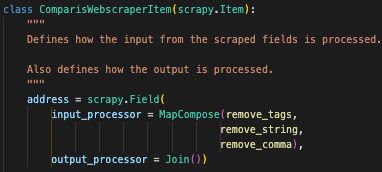
\includegraphics[width = 90mm]{prog_5.png}}
    \caption{Defining an Item}
    \label{fig:itemloader}
\end{figure}


% \begin{python}
% class ComparisWebscraperItem(scrapy.Item):
%     address = scrapy.Field
%         input_processor = MapCompose(remove_tags, 
%                                     remove_string, 
%                                     remove_comma), 
%         output_processor = Join()
% \end{python}\captionof*{python}{Test}

As a consequence the \pkg[ItemLoader] is created.
\pkg[Scrapy] provides the user with six different input processors,
including  \pkg[MapCompose()] which was used extensively.
These work like normal functions \cite{sDemystifyingScrapyItem2020}.
If need be, custom functions can be added, which was also done numerous times in this project.

For illustration purposes we provide figure \ref{fig:itemloader}. 
There the definition of a field in the \pkg[ItemLoader] can be seen in action.

When scraping an \acs*{html} field, there are two broad scenarios:
\begin{enumerate}
    \item The field is available on every website's \acs*{html}
    \begin{itemize}
        \item This is the case with fields that contain price, square meters or address for example
    \end{itemize}
    \item The field is only available sometimes
    \begin{itemize}
        \item …and is of categorical nature (e.g. \textit{"Does the property have a washing machine (Yes/No)?"})
        \item …has content that needs to be scraped (e.g. the construction year, if present, will be scraped)
    \end{itemize}
\end{enumerate}

When scraping the field "address" (scenario $1$ applies) several input- and output processors are defined (see figure \ref{fig:itemloader}).
The input processor is primarily \pkg[MapCompose()] and \pkg[remove\_tags.]
The latter is technically a function and is imported from the \pkg[w3lib.html] library.
In figure \ref{fig:itemloader} \pkg[remove\_string] and  \pkg[remove\_comma] can also be seen.

\begin{figure}[htbp]
    \centerline{
        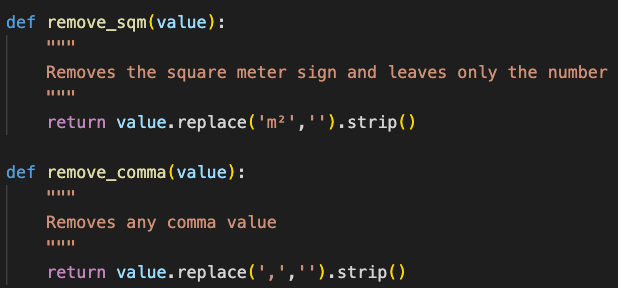
\includegraphics[width = 85mm]{prog_18.png}}
    \caption{Function for fields that are not always present}
    \label{fig:remove_string}
\end{figure}

They are instances of custom functions that were defined manually 
in the \pkg[items.py] file during the process of scraping.
As with the \pkg[remove\_tags] they can then be passed to the \pkg[MapCompose()] processor.
This worked very well for fields which were always present (i.e. price, address, square meters etc.).

Fields that are not always present
(e.g. fields that state whether the apartment is equipped with a washing machine or not)
present an additional challenge  when scraping.
This seemingly complicated problem can be resolved quickly with a few lines of code:

\begin{figure}[htbp]
    \centerline{
        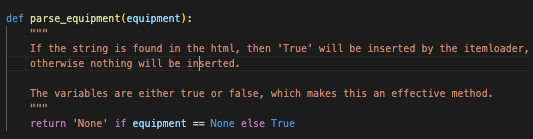
\includegraphics[width = 90mm]{prog_6.png}}
    \caption{Function for fields that are not always present}
    \label{fig:ispresentornot}
\end{figure}

Here the properties of both the XPATH and the functions are leveraged.
The XPATH of a given field, for example the one for the "elevator" field, 
will only return a result when it finds the keyword "\textit{Ascenseur}" within a specific range of the \acs*{html}.
Given this property of the XPATH and given that the keywords are always the same, 
it is natural to write a function that can evaluate this binary problem.
The function in figure \ref{fig:ispresentornot} returns \pkg[True] when the keyword is found,
and an empty value \pkg[(N/A)] otherwise.

By importing the class \pkg[ComparisWebscraperItem] into the \pkg[comparis\_scraper.py] file, the \pkg[ItemLoader] 
could be put to use.

\subsection{Implementation of the \ac{gui}}
\subsubsection{Organizing the scraped data}
The first step to building the \ac{gui} is organizing the data that was obtained from the scraping.
For this step we use the same program as in our sister project in "Advanced Data Analysis", named \pkg[cleaning\_database\_\ac{gui}.py].
We first analyze the two separate datasets that we obtained from the scraping. 
These are named \pkg[property\_codes.csv] and \pkg[property\_details.csv].
We analyze them by printing the headings and the description to check the data and the types.
We then merge them. After this, we sort through the values, removing all the missing variables and errors. 
We create dummy variables for the variables that might be interesting for graphs or regression analysis.
We then proceed to split the address from the ZIP code, to get the ZIP code in a separate column. 
We do this as we do not have precise addresses and we want to be able to search properties within a certain ZIP code. 
Finally, we drop the variables that are not needed and save the sorted data into the excel file \pkg[/\ac{gui}/data.xlsx].
This will be the dataset we use for our \ac{gui} program. \par
We also create a short program named \pkg[graphs\_\ac{gui}/.py] to prepare the data for the graphs 
we will want to display on the interface. We use the excel file we have just created named \pkg[data.xlsx].
We first drop all the variables we do not want to keep. 
We then group the remaining variables, for a given category, such as ZIP code and number of rooms, by average price.
We save these grouped datasets into two separate excel files, namely \pkg[MeanPriceRooms.xlsx] and \pkg[PricebyZip.xlsx] in the \ac{gui} folder.
These last datasets will only be used for the graphs.\par

\subsubsection{Building the \ac{gui}}
To build the \ac{gui} we created a new program named \pkg[main5.py].
We first defined what the \ac{gui} was supposed to do.
We decided, we wanted the user to be able to search for a property within a certain price range, 
or with a specific number of rooms or within a specific ZIP code. We also wanted to display graphs for general information.
Thefore to build this \ac{gui} we needed to have different tabs to search for these separately.
We also needed to be able to clear the search to be able to run the program multiple times. \par
To start the program that will create the interface, we start by defining the characteristics of the root widget otherwise referred to as the main window,
such as height, width and title. We then add the notebook instance to add tabs to the interface.
In \pkg[tkinter], these are knows as frame widgets. From there, we format the frames and add the labels, entries and buttons we wish to have in each tab. 
For the formatting we chose to use the grid method. This defines the place of each item, also called widget, within the frame based on colums and rows.
The grid manager automatically adapts the size of grid based on the number of widgets inside the frame. 
We then add the scrollbar to the root window to be able to scroll through the returned properties if the list is long. 
We also add a treeview instance so that the pulled data from the dataset is displayed in a hierarchical and tabular structure. 
Finally we define the functions. We use three main functions, one to search through the database and retrieve the data to the interface. 
The second function to clear the search and delete the displayed data. The last function creates and displays the graphs. 
Each function is adapted to the chosen variable, such as price, number of rooms or ZIP code to display the correct information.\par
This is a very basic \ac{gui} to make it easier for the user to interact with the scraped data.
The aim would be to develop the interface to handle searches that are more complex, such as conditional searches with more than one characteristic.
More graphs could also be displayed to give diverse information to the user. 
See the outlined workflow as a flowchart on the right-hand side in figure \ref{fig:flowchart1}.

\begin{figure}
    \begin{tikzpicture}[auto, node distance = 4mm and 6mm, start chain = going below]
        \begin{scope}[nodes={on chain, join=by line}]
            \node[startstop] (start) {Start};
            \node[startstop] (in1) {Load Scraped data};
            \node[decision] (dec1) {Is Data Cleaned?};
            \node[startstop] (in2) {Start GUI by importing tkinter};
            \node[process] (pro2a) {link to cleaned dataset};
            \node[process] (pro2) {Format main window};
            \node[process] (pro3) {Format frames as tabs};
            \node[process] (pro4b) {Create functions for each tab};
            \node[process] (pro5) {Define main loop};
            \node[decision] (dec2) {Check GUI is working};
            \node[startstop] (in3) {User can search properties};
            \node[decision] (dec4) {End the program?};
            \node[startstop] (start1) {End};
            %%%%%%%%%%%%%
        \end{scope}
        \begin{scope}
            \node[process, left=of dec1] (pro1) {Clean and Organize data};

            \node[process, left=of dec2] (pro6) {Find bug};

            \node[process, left=of dec4] (pro7) {Re-run the program};

            
            \draw [->, left of = dec1] (dec1)  -- node[yshift=0.3cm, text width= 0.2cm]
                                    {\textcolor{red}{No}}
                                    (pro1);

            \draw                   (dec1) -- 
                                    node[yshift=0.1cm, text width= 0.2cm]
                                    {\textcolor{ForestGreen}{Yes}}
                                    (in2);

            \draw [->] (dec2) -- node[yshift=0.5cm, text width= 0.2cm]
                                    {\textcolor{red}{No}}
                                    (pro6);
            % Yes Node
            \draw                   (dec2) -- 
                                    node[yshift=0.1cm, text width= 0.2cm]
                                    {\textcolor{ForestGreen}{Yes}}
                                    (in3);
            % No Node
            \draw [->, left of=dec4] (dec4) -- 
                                    node[yshift=0.3cm, text width= 0.2cm]
                                    {\textcolor{red}{No}}
                                    (pro7);
            % Yes Node
            \draw                   (dec4) -- 
                                    node[yshift=0.1cm, text width= 0.2cm]
                                    {\textcolor{ForestGreen}{Yes}}
                                    (start1);

            \draw [->, left of = dec1] (pro1) |-    (pro2);

            \draw[->, draw = blue] (pro6) |-  (in2);
            %\draw [->] (pro6) |-  (in2);
            \draw [->] (pro7) |-  (in3);
        \end{scope}
    \end{tikzpicture}

\caption{Workflow for Using the \acs*{gui}} \label{fig:flowchart1}
\end{figure}

\end{document}